% sets default font to Arial
\renewcommand{\rmdefault}{phv} % Arial
\renewcommand{\sfdefault}{phv} % Arial

\documentclass[11pt,a4paper,titlepage]{article}

\title{Can migratory behaviour be predicted from individuals' localised movements, within a commercial fishery area?}
\date{MRes CMEE Project Proposal}
\author{Supervisors:\\Dr. David Jacoby, Zoological Society of London\thanks{Primary Supervisor; contact: david.jacoby@ioz.ac.uk}\\Dr. Matias Braccini, Department of Fisheries, Western Australia\\Dr. Samraat Pawar, Imperial College London}

\usepackage{float}
\usepackage[left=2cm,right=2cm,top=2cm,bottom=2cm]{geometry}
\usepackage{pgfplotstable}
\usepackage{graphicx}
\usepackage{lineno}
\usepackage{natbib}
\linespread{1.5}




\begin{document}
	
	\maketitle
	
	\newpage
	\linenumbers	
	\section{Keywords}
	 
	Animal movement; Behavioural plasticity; Shark; Spatial networks; Acoustic telemetry; Fisheries management.
	
	\section{Introduction}
	
	\paragraph{}Studying the migratory behaviour of pelagic marine organisms poses one of the greatest challenges to movement ecology, due to the difficulty of data collection \cite{Jacoby2016}. Many of these species are at risk due to large scale fisheries \cite{Braccini2017,Braccini2018}, and ineffective management due to variability in organisms spatial and temporal range. Two such species are the sandbar shark (\textit{Carcharhinus plumbeus}) and the dusky shark (\textit{Carcharhinus obscurus}), both classified as vulnerable by the IUCN \cite{Musick2009,Musick2009a}. Moreover, the majority of studies focus on population movements, as opposed to individuals \cite{Jacoby2012}.
	
	\paragraph{}This study will focus on the relationship between localised and migratory movements of two species of shark, the Sandbar shark \textit{Carcharhinus plumbeus} and the Dusky shark \textit{Carcharhinus obscurus}. The study will investigate individual movements using acoustic detection data from a network of receivers in Western Australia . The three main questions that will be addressed using both species are: (1) whether residential movement behaviours within the network correspond to migratory behaviour; (2) whether migrations are cyclic, and movement is direct between breeding and resident habitats; (3) whether movements are stratified by biotic factors such as age and sex.
	
	
	\section{Proposed Methods}
	
	Analysis of the data will be conducted using R \cite{RCoreTeam2015}, using spatial network analysis to model individual movement behaviour \cite{Jacoby2016}. A residency index will be used to compare resident behaviour of individuals. 

	
	\section{Anticipated Outcomes}
	
	Work carried out in this area with dusky and sandbar sharks has been incredibly limited, therefore outcomes are difficult to predict. Dusky sharks have been shown, especially in females, to undertake a southerly migration in the breeding season \cite{Braccini2018}, however this has not been carried out with sandbar sharks, or with a network based approach.
	
	\section{Project Feasibility}
	
	\paragraph{}The data for this project has already been collected and provided by co-supervisor Dr Matias Braccini. The dataset contains just under 200,000 observations of the 127 tagged sharks, 59 of which are sandbar and 68 dusky, with spatial and temporal information for each detections, between 2011 and 2016 (potentially up to 2018). Guidance on analysis in R has been provided already, and Dr David Jacoby has offered to provide specific training on network analysis at ZSL. Guidance on applying the results to fisheries management will be provided by Dr Matias Braccini, in the department of fisheries, Western Australia. See Figure \ref{fig:gantt} for a detailed timeline of the project.

	
	\begin{figure}[h]
		\centering
		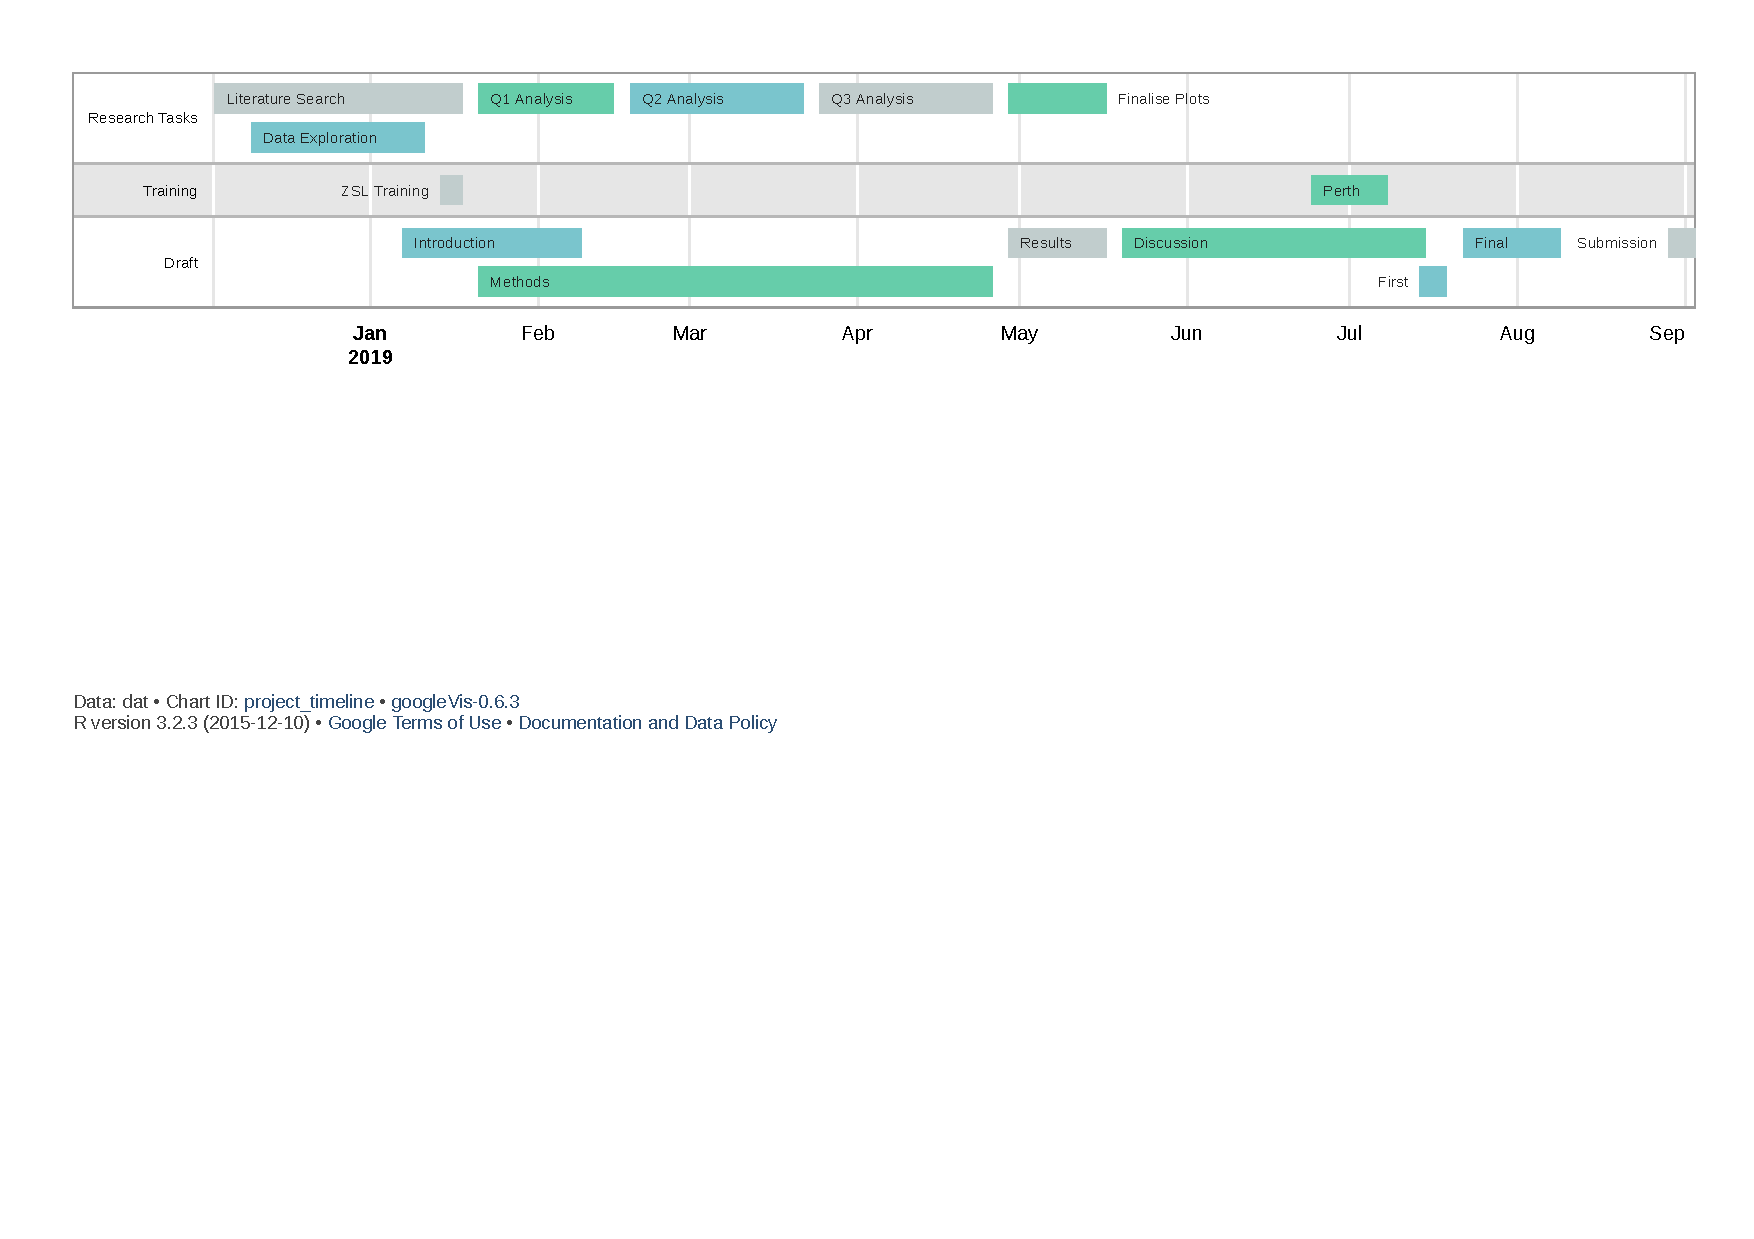
\includegraphics[width=\linewidth,trim={0 14cm 0 0},clip]{gantt.pdf}
		\caption{Proposed project timeline, where research tasks refer to actions carried out during the project; training refers to training provided by the supervisors: ZSL Training - Dr. Jacoby regarding network analysis and Perth - training with Dr Braccini in Perth, Western Australia, on application of results in fisheries management; and draft refers to drafting each section on the thesis, with first and final referring to complete drafts, before submission.}
		% label invisible but can be used to refer to figure in text
		\label{fig:gantt}
	\end{figure}
	
	\section{Budget}
	
	\begin{itemize}
		\item $\pounds$100 - Travel to ZSL offices for training in network analysis and fortnightly meetings with primary supervisor and his research team.
		\item $\pounds$750 - Travel to Perth, Australia, in June for training with co-supervisor Dr Matias Braccini, to help contextualise the project and ensure the research is applicable to fishery policy in the region.
		\item $\pounds$150 - Accommodation in Perth for visit.
	\end{itemize}

	\newpage
	\bibliography{projectproposal.bib}
	\bibliographystyle{plainnat}
	
	
	\newpage
	
	\section{Supervisor Approval}
	
	\paragraph{}\textbf{I have seen and approved the proposal and budget.}

	\paragraph{}Name:
	
	\paragraph{}Signature:
	
	\paragraph{}Date:
	
\end{document}